\subsubsection{Operational Setup}
\label{sxn:ST_OP_setup}
\begin{figure}
%  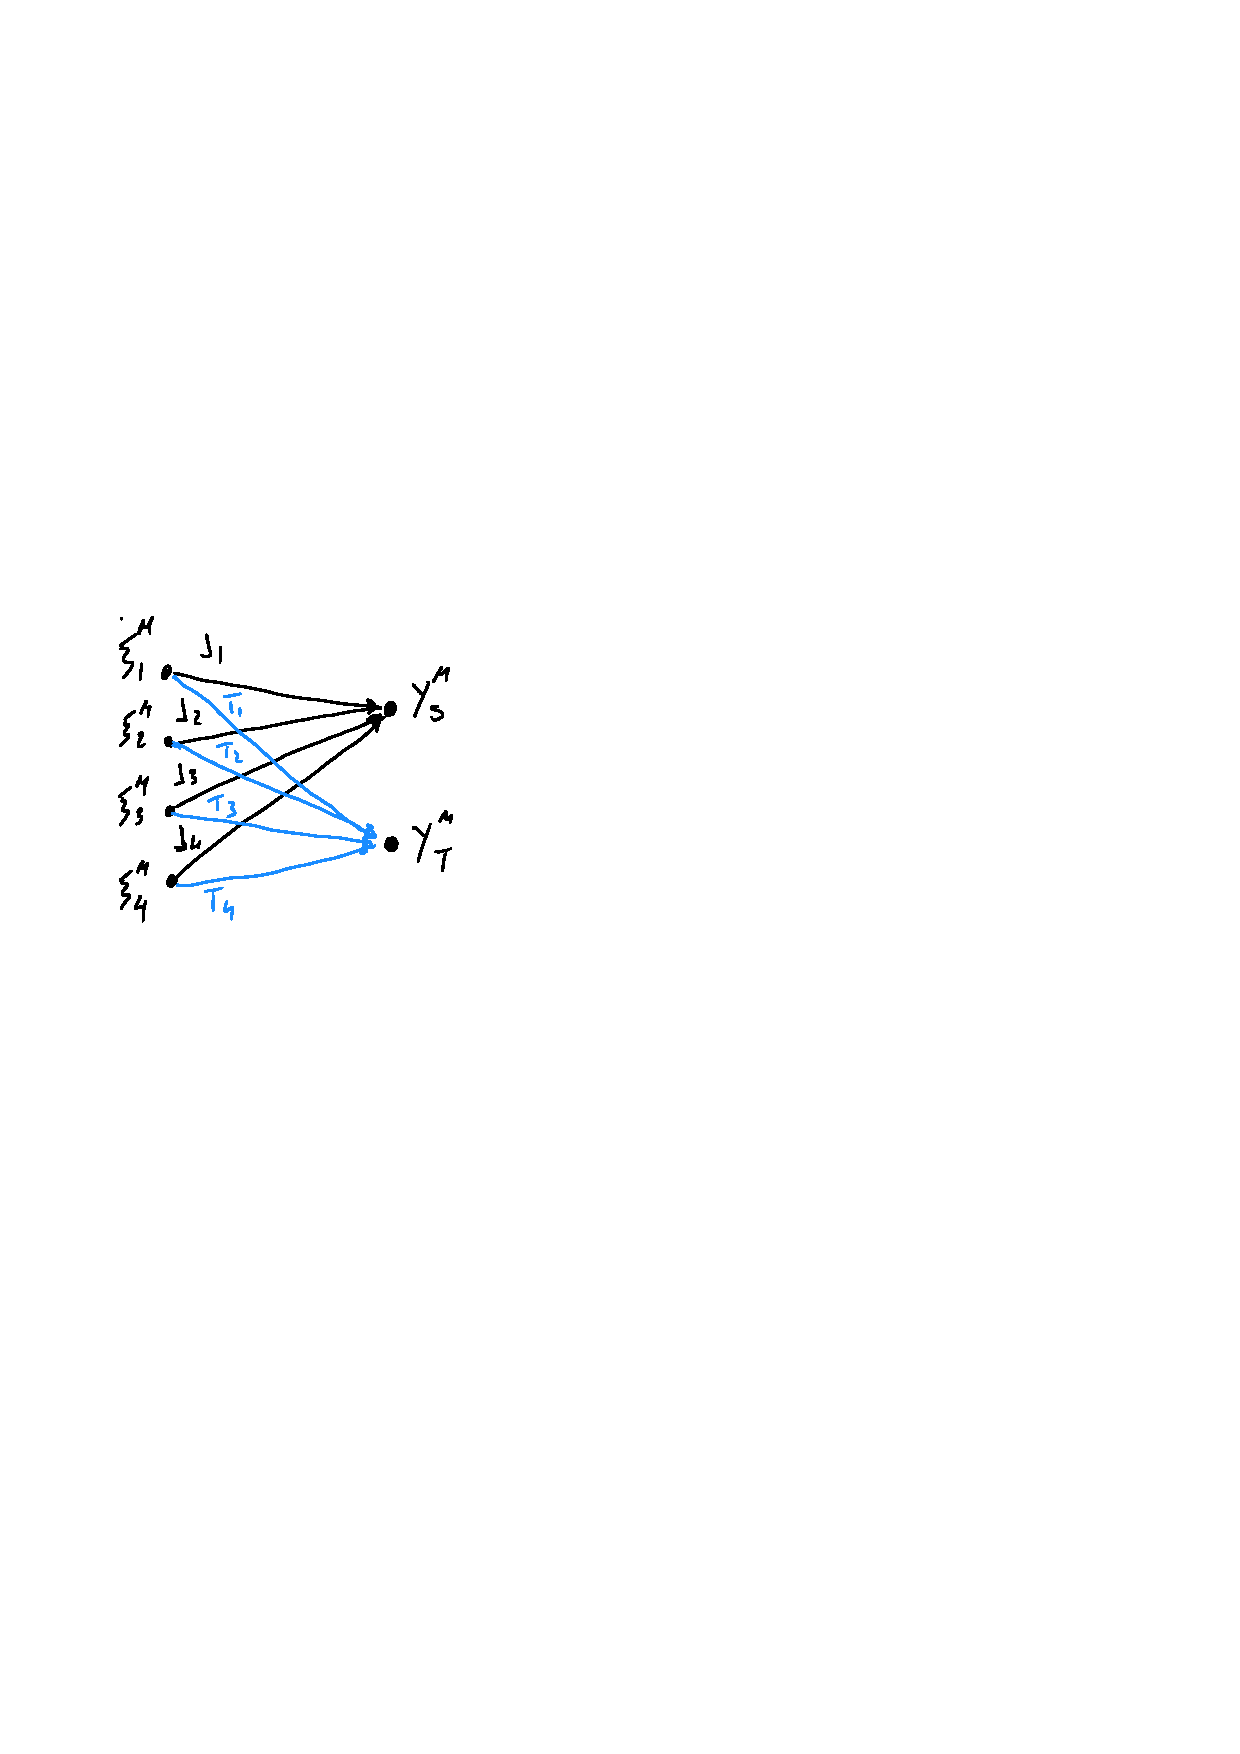
\includegraphics[width = 0.3\textwidth]{./img/perceptron.pdf}
  \begin{center}
    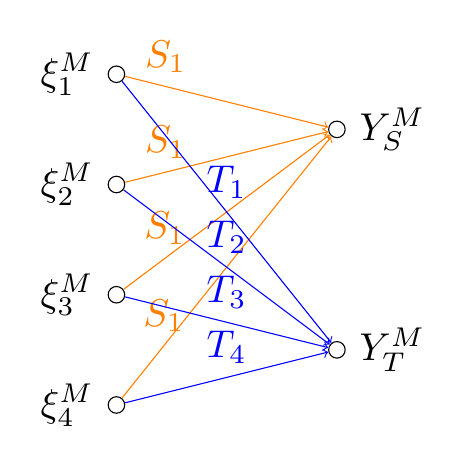
\begin{tikzpicture}[scale=1.4, every node/.style={transform shape}]
    \node[draw, circle, minimum size=0.15cm, inner sep=0.05cm] (A) at (0, 3) {};
    \node[draw, circle, minimum size=0.15cm, inner sep=0.05cm] (B) at (0, 2) {};
    \node[draw, circle, minimum size=0.15cm, inner sep=0.05cm] (C) at (0, 1) {};
    \node[draw, circle, minimum size=0.15cm, inner sep=0.05cm] (D) at (0, 0) {};

    \node[left] at (A.west) {$\xi_1^M$};
    \node[left] at (B.west) {$\xi_2^M$};
    \node[left] at (C.west) {$\xi_3^M$};
    \node[left] at (D.west) {$\xi_4^M$};

    \node[draw, circle, minimum size=0.15cm, inner sep=0.05cm] (Y) at (2, 2.5) {};
    \node[draw, circle, minimum size=0.15cm, inner sep=0.05cm] (Z) at (2, 0.5) {};

    \node[right] at (Y.east) {$Y_S^M$};
    \node[right] at (Z.east) {$Y_T^M$};
  
    % Arrows
    \draw[->, orange] (A) -- (Y) node[pos=0.2, above] {$S_1$};
    \draw[->, orange] (B) -- (Y) node[pos=0.2, above] {$S_1$};
    \draw[->, orange] (C) -- (Y) node[pos=0.2, above] {$S_1$};
    \draw[->, orange] (D) -- (Y) node[pos=0.2, above] {$S_1$};

    \draw[->, blue] (A) -- (Z) node[pos=0.5, above] {$T_1$};
    \draw[->, blue] (B) -- (Z) node[pos=0.5, above] {$T_2$};
    \draw[->, blue] (C) -- (Z) node[pos=0.5, above] {$T_3$};
    \draw[->, blue] (D) -- (Z) node[pos=0.5, above] {$T_4$};

  \end{tikzpicture}
  \end{center}
  \caption{Pictorial representation Student and Teacher Perceptrons.}
\end{figure}



Here, describe the basic setup of the classic \StudentTeacher model, taking an operational view from the perspective of a practitioner training real-world \Student and \Teacher models.  Specifically, we present the \AnnealedApproximation (AA) in a practical light,
and use it explain the difference between computing the \emph{Empirical \GeneralizationError}, $\AVGEMPGE$, for the \emph{\TrueAccuracy}
and for the \emph{\Precision} of a \Teacher model. Table~\ref{tab:st_notation} summarizes some of the key notation we will be using in this section.
\begin{table}[h]
\centering
\begin{tabular}{@{}ll@{}}
\toprule
\textbf{Symbol} & \textbf{Meaning} \\
\midrule
$T$                      & Teacher model (fixed network) \\
$S$                      & Student model (trained to mimic $T$) \\
$\ADD$             & True dataset of $(\DATA,\Ytrue)$ pairs \\
${\mathcal D}$ & Gaussian‐field idealization of $\mathcal D$ \\
$ \AVGGE^{emp}$    & Average empirical test‐set error estimate \\
 $\AVGGE^{T}$          & Average, true generalization error of $T$ (unknown) \\
$\AVGGE^{ST}$       & Student–Teacher average generalization error \\
$\SVEC,\;\TVEC$                      & Student and Teacher weight vectors \\
$\Ys,\;\Yt$                      & Student and Teacher labels $(+1|-1)$  for example $\mu$\\
$\AVGR$                      & Student-Teacher  Overlap $\displaystyle \AVGR=\SVEC^\top \TVEC$ \\
$\epsilon(R)$            & \EffectivePotential (i.e.,\ $1-\AVGR$) \\
$\eta(\SVEC,\TVEC)$            & \SelfOverlap (i.e., $\AVGR$) \\
$\Q^{ST}$            & Student-Teacher Perceptron \Quality \\

\bottomrule
\end{tabular}
\caption{Key notation for our formulation of the Student–Teacher model.}
\label{tab:st_notation}
\end{table}


\paragraph{Test Error of the Teacher}

We start by describing how to obtain a simple formal expression for the empirical test errors of the \Teacher, first for the \TrueAccuracy.

Let us say we have a model, called \Teacher $(T)$, which maps some \emph{actual} (i.e., correlated) data
$\DATA\in\ADD$ to some known or \emph{true}  labels $(\Ytrue)$
(where,  $\Ytrue$ is, say, an $N$-dimensional vector of binary labels).
We might say that $\Ytrue$ represents the \emph{\GroundTruth} for the problem.
Operationally, we train the \Teacher $T$ to reproduce or at least approximate the true labels $\Ytrue$.
\begin{align}
 T:\DATA\rightarrow \Yt \approx \Ytrue.
\end{align}
If $T$ reproduces the true labels exactly, we might say that the \Teacher has been
trained to \emph{\Interpolation}, and therefore, $\Yt = \Ytrue$.
Indeed, most models today are trained to \emph{\Interpolation}, and we don't need to
necessarily worry about the difference between the true and the predicted \Teacher labels.
Formally, however, and to understand better the \AA, it is beneficial to discuss the implication
of this distinction.

Following \EQN~\ref{eqn:dnn_energy}, lets say the \Teacher outputs are specified
by an  Energy function $E^{T}_{NN}$
\begin{align}
\label{eqn:T_ENN}
\Yt=E_{NN}(T,\DATA) 
\end{align}
\footnote{Do not confuse the Energy/output function $E_{NN}$ with the energies $\mathbf{\Delta E}$  defined below to represent the ST error function(s).  We refer to outputs of $E_{NN}(\TVEC,\DATA )$, when applied to a data point $\DATA$, as energies because they are effectively un-normalized probabilities for the class outputs (for labels $\Ymu=1$ or $-1$).  }
so that we may write the \emph{Empirical} \AverageTrainingError
$\AVGEMPTE$
as 
\begin{align}
\label{eqn:Eg_train}
\AVGEMPTE:= \frac{1}{N^{train}}\sum_{\mu=1}^{N^{train}}\mathcal{L}[\Ytrain,E_{NN}(T,\DATAtrain)]  .
\end{align}
Ideally, we seek the \emph{True} \AverageGeneralizationError of the \Teacher, denoted  $\AVGGE^{T}$. 
Of course, this is unknowable, but in practice, we estimate $\AVGGE^{T}$ 
by measuring the error of the \Teacher predictions on some test (or hold-out) set $(\DATA^{test}, \MY^{test})$.
We call this the \emph{Empirical \AverageGeneralizationError}, $\AVGEMPGE$, and write
\begin{align}
\label{eqn:Eg_test}
 \AVGGE^{T}\approx \AVGEMPGE:= \frac{1}{\Ntest}\sum_{\mu=1}^{\Ntest}\mathcal{L}[\Ytest,E_{NN}(T,\DATAtest)] .
\end{align}
To measure the error, the loss function $\mathcal{L}$ may be a L1 $(\ell_1)$ or L2 $(\ell_2)$ loss;
whereas for training a model, it is usually something like a cross-entropy loss, but this detail does matter later.

If we don't have a hold-out set, however, we can still estimate $\AVGGE^{T}$ using the \Student-\Teacher approach.

\paragraph{Estimating the Student-Teacher Error: Accuracy vs. Precision}
Imagine we train a Student model $S$ (with the same architecture as the Teacher $T$) on the dataset $\mathcal D$, using $T$'s outputs as targets:
\begin{equation*}
S: \mathcal D \to y^{S}_\mu \approx y^{T}_\mu,
\label{eqn:S_ENN}
\end{equation*}
where $y^T_\mu = E_{NN}(T, x_\mu)$ are the Teacher’s predicted labels or energies.


\begin{figure}[ht] % [h] places the figure approximately here
  \centering
  \resizebox{0.75\textwidth}{!}{

\begin{tikzpicture}

    % Axis
%    \draw[->] (0,0) -- (0,4) node[left] {Predictions};
    \draw[->] (0,0) -- (6,0) node[below] {Value};
    
    % Gaussian distribution
    \draw[thick, red] plot [smooth] coordinates {(1,0) (2,1) (3,3) (4,1) (5,0)};
    
    % Ground Truth line
    \draw[thick, blue] (3,0) -- (3,3.2);
    \node[blue, above] at (2.5,3.2) {\textbf{Accuracy} };
    \draw[->] (2.5,3.) -- (3,3.);
    \node[black, below] at (0.75,3.2) {\textbf{Teacher output} $\Yt$};

    % Accuracy bracket
    \draw[<->, blue, thick] (3,3.2) -- (4,3.2);
    
    % Teacher (high accuracy, low precision)
    \fill[darkgreen] (4,3) circle (0.15);
    \node[right, below] at (5.5,2.9) {\textbf{Ground truth} $\Ytrue$};
    
    % Student outputs (spread)
    \draw[->] (2.5,1) -- (3.5,2);
    \node at (0.75,0.75) {\textbf{Student outputs} $\Ys$};

    % Precision label
    \draw[<->, red, thick] (1,-0.5) -- (5,-0.5);
    \node[red, below] at (3,-0.5) {\textbf{Precision}};
    
    % Bullseye diagram (Right side)
    \begin{scope}[xshift=9cm, yshift=2cm]
        \draw[thick] (0,0) circle (1.8);
        \draw[thick, fill=white] (0,0) circle (1.2);
        \draw[thick, fill=white] (0,0) circle (0.6);

        \fill[blue] (-0.5, 0.0) circle (0.10);
        % Random student outputs
        \foreach \x/\y in {-0.6/0.3, 0.1/-0.7, -0.15/0.5, -0.3/-0.5, -0.75/0.75, -0.9/-0.2} {
            \fill[red] (\x,\y) circle (0.08);
        }
        
        % Teacher dot in center
        \fill[darkgreen] (0,0) circle (0.15);
        
        \node[left] at (2.,-2.5) {\textbf{Bullseye Example}};
    \end{scope}

\end{tikzpicture}
  }
  
\caption{Precision vs. Accuracy}
 \label{fig:precision}
\end{figure}


Figure~\ref{fig:precision} illustrates the following two scenarios side by side:
\begin{itemize}
  \item \textbf{Accuracy (Interpolation) regime:}
    If $T$ perfectly interpolates the true labels ($y^T_\mu = y^\text{true}_\mu$), then
    \( \|y^S_\mu - y^T_\mu\| = \|y^S_\mu - y^\text{true}_\mu\| \)
    measures how well the student recovers the Ground Truth labels—i.e., the Student's \emph{training accuracy}.

  \item \textbf{Precision (Noisy teacher) regime:}
    If $T$ itself makes mistakes ($y^T_\mu \neq y^\text{true}_\mu$), then
    \( \|y^S_\mu - y^T_\mu\| \)
    estimates how faithfully $S$ reproduces $T$ (its precision), rather than true accuracy.
\end{itemize}

By analyzing the Student–Teacher overlap $R = \sum_\mu s^T t$, one can show that the average generalization error of $T$ depends simply on $1-R$ under the annealed approximation—-even when $S$ was trained on noisy labels. In practice, we exploit this fact by training a large ensemble of students to estimate $R$ and hence recover the teacher’s true error.
%\paragraph{Estimating the Teacher Error with Students: Accuracy vs. Precision}
%
%Imagine training a \Student $(S)$  model (with a similar architecture as $T$, and acting on the same  
%dataset $\DATA\in\ADD$), which tries to  reproduce the \Teacher predictions:
%\begin{align}
%S:\DATA\rightarrow \Ys \approx \Yt  ,
%\end{align}
%and assume the \Student outputs $\Ys$ are given by the Energy output function $E^{S}_{NN}$
%\begin{align}
%\label{eqn:S_ENN}
%\Ys=E_{NN}(S,\DATA) ,
%\end{align}

%If the \Teacher is trained to \Interpolation, then the difference between
%the \Student and the \Teacher labels 
%estimates the true error, i.e., $\Vert\Ys-\Yt\Vert=\Vert\Ys-\Ytrue\Vert$,
%and this error is associated with the \TrainingAccuracy of the model in predicting the \GroundTruth.
%But if the \Teacher makes some errors, then $\Vert\Ys-\Yt\Vert$
%is now estimating the \Precision of the model.
%These two situations are depicted in Figure~\ref{fig:precision}.
%
The \StudentTeacher model also explains why NNs can generalize even when trained to \Interpolation on noisy data (which has been a source of confusion \cite{Understanding16_TR}). In this model, the \GeneralizationError $\AVGGE^{T}$ is a simple function of the overlap $R$ between the \Teacher $T$ and the \Students $S$, i.e., $\AVGGE^{T}\sim \THRMAVG{1-\EPSLR}$. So even if the \Teacher $T$ is trained on noisy data, as long as there are \Students $S$ with significant overlap $R$ with the \Teacher, the \Teacher \GeneralizationError $\AVGGE^{T}$ can be considerably small. For more details, see \cite{MM17_TR_v1}


\paragraph{Learning the Student}
Moving forward, we will always assume the \Teacher is trained to \Interpolation because this
actually corresponds to the \AnnealedApproximation, whereas if the \Teacher makes
errors, we may need to consider \Quenched averages, explained below.

Imagine now that in order to estimate the empirical \AverageGeneralizationError, $\AVGEMPGE$,
by training a very large number of Students, and computing the average ST error on some test set.
Let us break the data set into training $\DATAtrain$ and test $\DATAtest$ examples, 
train models on the training data (that is, find the optimal model weights), 
and evaluate the $S$ and $T$ models on the test data.

The \Student learning task can be written as in \EQN~(\ref{eqn:dnn_opt})
as the following optimization problem over the training data:
\begin{align}
\underset{\{S'\}}{\argmin}\sum_{\mu=1}^{N^{train}}\mathcal{L}[E_{NN}(S',\DATAtrain),E_{NN}(T,\DATAtrain)]   ,
\label{eqn:ST-learning-task}
\end{align}
%Notice that, at this step, the \Student $S$ and the \Teacher $T$ both depend explicitly on the specific choice of the training data $\DX_{train}$.  
%That is, we could write $S[\DX^{train}], T[\DX^{train}]$.

If the \Teacher is trained to \Interpolation, then the NN optimization problem 
training a \Student to reproduce the \GroundTruth labels, so that $\Ys\sim y_{\mu}^{true}$
for both the training and test sets.
\begin{align}
\underset{\{S'\}}{\argmin}\sum_{\mu=1}^{N^{train}}\mathcal{L}[E_{NN}(S',\DATAtrain),\Ytrue]   ,
\label{eqn:ST-learning-intepolation}
\end{align}

But if not, then the \Student is reproducing the possibly
incorrect \Teacher labels, and, importantly, the \Student $S$ now depends explicitly
on how the \Teacher was trained.  That is, we should denote that the learned
\Student explicitly depending on $T$, i.e. $S\rightarrow S[T]$.
This will be important below.

\paragraph{The \AverageGeneralizationError}
In either case, however, we may still estimate the Empirical \AverageGeneralizationError
by replacing the test predictions in \EQN~\ref{eqn:Eg_test} with the student predictions
$y_{\mu}^{test}\rightarrow \Ys$, and then averaging directly over the test data $\DATAtest$
for all possible or available test examples.

If we have a very large number of suitable Students
(say, drawn from some random distribution), then we can try to estimate the 
\AverageGeneralizationError of the \Teacher, i.e., $\TGE^{T}\approx\AVGEMPGE$.
$\AVGEMPGE$ is given by an average loss, the average is 
over all possible Students $N_S$,  and then  over all  $\Ntest$ test data points $\DATAtest\in\mathbf{D}$ 
\begin{align}
  \AVGEMPGE
  &=
  \frac{1}{\Ntest}\sum_{\mu=1}^{\Ntest}
  \frac{1}{N_S}\sum_{S}
  \mathcal{L}[E_{NN}(S,\DATAtest),E_{NN}(T,\DATAtest)]  \\ \nonumber
    &=
  \frac{1}{N_S}\sum_{S}
    \frac{1}{\Ntest}\sum_{\mu=1}^{\Ntest}
    \mathcal{L}[E_{NN}(S,\DATAtest),E_{NN}(T,\DATAtest)] ,
\label{eqn:emp_gen_error}
\end{align}
where (ideally) $\Ntest$ is extremely large.

In Bra-Ket notation, we may also write
\begin{align}
  \AVGEMPGE
  &= \langle \langle \DETOPSTx \rangle_{S} \rangle_{\DXtest}\\ \nonumber
  &= \langle \langle \DETOPSTx \rangle_{\DXtest} \rangle_{S}
\end{align}
where $\DETOPSTx:=\mathcal{L}[E_{NN}(S,\DATAtest),E_{NN}(T,\DATAtest)]$.
For the empirical estimate, it does not matter what order we take the sums in,
but we are not estimating the
the True \AverageGeneralizationError  of the \Teacher, $\AVGGE^{T}$,
unless $T$ is trained to \Interpolation.
For the theoretical estimate, however, the order can be important, and this also depends on
if $T$ is trained to \Interpolation or not.
\footnote{This approach can be likened to the Bootstrap method~\cite{efron1993bootstrap} used for error estimation.  However, the Bootstrap method predominantly emphasizes variations in the input data $\NDX\in\mathbf{D}$, while in this context, we are essentially bootstrapping over the students $S$.}

%\michael{Is this for the optimal values of the parameters in the learning task \EQN~(\ref{eqn:student-learning-task})%?  Presumably not, since we are averaging? }
%\charles{Good question. We do not specify how the hyperparameters are selected.}

\paragraph{Annealed vs. Quenched Averages}
Recall that in the \STATMECH approach to computing errors, we do not break the data into
training and test, but, instead, to obtain the \AverageGeneralizationError, $\AVGGE$, use
the \GeneratingFunction approach. In doing this, we need to compute both the \ThermalAverage
over the model weights ($S,T$), and also take the data average over the entire available model data set $\MDD$
And the order can matter.

In the case where the \Teacher is trained to \Interpolation, may train the \Student 
independently of \emph{when} the \Teacher.  
But if \Teacher is \emph{not} trained to \Interpolation, then formally we must train the \Teacher
first to obtain target predictions for the \Student.  That is, the \Student formally
depends on the \Teacher, $S[T]$.
The empirical errors in $T$ would then formally depend on the specific instantiation of the data  $\NDXIn\in\MDD$,
and therefore, conceptually imagine that we must first average over the data
before averaging over the weights.
\emph{Training to \Interpolation} corresponds conceptually to working with a model
in the \AnnealedApproximation, whereas not doing so corresponds to \Quenched case.

Practically, when the \Teacher is not trained to \Interpolation, 
we may need to resample the training data and training an ensemble of models to compensate for anomalies in training data (bad labels, noise, etc.) that may cause the underlying model to overfit to the training data.
Theoretically, within \SMOG, this is equivalent to \emph{quenching} the system to the data (a term analogous to quickly cooling a physical system, frezing in any defects).
In contrast, when one \emph{anneals} a physical system, one heats up and cools it down slowly, and repeatedly, thereby removing any defects (of data anomalies for NNs, or material defects in a physical system).

In \STATMECH, one can perform a so-called quenched average using a replica calculation,
effectively removing the dependence on test and/or training data
from the final estimate for $\AVGEMPGE$.
However, the theoretical quenched result may differ significantly from the annealed case when the underlying model is unrealizable~\cite{SST92}. 
This may occur when the training data is very noisy and/or the model architecture is such that it can not correctly predict all the training labels.
In such cases, the model will always have some finite, non-zero Average \TrainingError, $\AVGTE > 0$,
even in the \LargeN limit of infinite data $\ND=\infty$. In such a case, this indicates
a highly complex error landscape with many local minima separated by extremely high barriers,
and a slowing down of the dynamics.%
\footnote{In modern ML parlance, one might say the model can not be evaluated at interpolation, although 
in practice such a model might have a zero empirical \TrainingError since it may overfit the specific training data.}
\michael{This seems like important discussion, but it is related to what is going on in Section~\ref{sxn:SMOG_main-spin_glass}; I feel like we should have a minimalistic discussion of things like spin glasses in the main text, and then have a self-contained appendix that goes into it in more detail, since it gets in the way of getting to Section~\ref{sxn:SMOG_main-st_av} and Section~\ref{sxn:matgen}.  }
\charles{This is a minimal discussion.  }

While it is commonplace to train ensembles and/or use cross-validation when training small models (as the above discussion assumes),
this could be extremely expensive and impractical in modern ML, e.g., for very large models like Large Language Models (LLMs).
For such massive NNs, one needs a theory that can detect anomalies in training directly from observations during and/or after training.
This is a hallmark of the \SETOL approach, and it distinguishes \SETOL from the classic \STATMECH approach.


\paragraph{Generalization Gap vs. Model Quality}
\label{sxn:SMOG_main-model_quality}

We should distinguish between what is typically done in the \SLT literature versus the \STATMECH approaches.
In \SLT, one is typically interested in modeling the \emph{\GeneralizationGap}.
The \GeneralizationGap quantifies the difference between a models performance on training data versus unseen test data:
\begin{align}
  \label{eqn:gen_gap}
  \mathcal{E}^{emp}_{gap}:= \TTE[\DXtrain]- \TGE[\DXtest]
\end{align}
In contrast, in \STATMECH approaches, one considers the \ModelGeneralizationError directly,
which is sometimes called the \ModelQuality in the \SLT literature.
\michael{I think SST looks at generalization error also.  I think this dichotomy isn't quite correct, and it convovles several issues.  It seems most connected with the par around \EQN~\ref{eqn:Qdef} and \EQN~\ref{eqn:GammaQdef}. Maybe we should combine this with that and put is somewhere, removing the incorrect claim/suggestion, and highlighting the ideas in the next par, which are key.
}
\charles{Thats not what this is about.  This is an important section that belongs here.
needs some work}
Model quality is an indication of the models accuracy, precision, recall, or any other relevant metric based on the task at hand.
%Here, we mean that the \ModelGeneralizationError is a measure of the \ModelQuality on such OOD data.

While related, in developing an analytic theory, the \GeneralizationGap and
the \ModelQuality (or \ModelGeneralizationError) require conceptually different approaches.
This is because the  \GeneralizationGap depends on a specific realization of the training data,
whereas our \ModelGeneralizationError will be formulated on a random training data set
(and then corrected later with empirical data).
In this sense, any theory of the \GeneralizationGap  requires a formalism where the
predicted model error is \Quenched to the training data, which is not what we want.
In contrast, the \ModelGeneralizationError  will be formulated using the \AnnealedApproximation (AA),
and is therefore both conceptually and mathematically simpler.
\michael{These ideas seem key; they should either be combined with the par around \EQN~\ref{eqn:Qdef} and \EQN~\ref{eqn:GammaQdef}, or they should be in the intro.}

\nred{Comment on our paper with YQ}



